\documentclass[11pt]{article}

\usepackage[letterpaper,margin=0.68in,headheight=15pt,footskip=28pt]{geometry}
\usepackage[T1]{fontenc}
\usepackage{lmodern}
\usepackage{microtype}
\usepackage{amsmath,amssymb}
\usepackage{booktabs,tabularx,array,multirow}
\usepackage{enumitem}
\usepackage[table]{xcolor}
\usepackage{tikz}
\usetikzlibrary{positioning,arrows.meta}
\usepackage[most]{tcolorbox}
\usepackage{multicol}
\usepackage{titlesec}
\usepackage{fancyhdr}
\usepackage{lastpage}
\usepackage{needspace}
\usepackage[hidelinks]{hyperref}

\definecolor{Navy}{HTML}{15324A}
\definecolor{Teal}{HTML}{118A8A}
\definecolor{Sky}{HTML}{DFF3F4}
\definecolor{Gold}{HTML}{F2B134}
\definecolor{GoldLight}{HTML}{FFF4D6}
\definecolor{Coral}{HTML}{E76F51}
\definecolor{CoralLight}{HTML}{FCE8E2}
\definecolor{Ink}{HTML}{24323D}
\definecolor{SoftGray}{HTML}{F4F6F7}
\definecolor{MidGray}{HTML}{667782}
\definecolor{AnswerBlue}{HTML}{1E5AA8}
\definecolor{Green}{HTML}{3A8D5D}

\color{Ink}
\setlength{\parindent}{0pt}
\setlength{\parskip}{4pt}
\setlist[itemize]{leftmargin=1.35em,itemsep=2pt,topsep=3pt}
\setlist[enumerate]{leftmargin=1.65em,itemsep=5pt,topsep=4pt}
\renewcommand{\arraystretch}{1.22}

\titleformat{\section}{\Large\bfseries\color{Navy}}{}{0pt}{}[\vspace{-3pt}\color{Teal}\titlerule]
\titleformat{\subsection}{\large\bfseries\color{Teal}}{}{0pt}{}
\titleformat{\subsubsection}{\normalsize\bfseries\color{Navy}}{}{0pt}{}
\titlespacing*{\section}{0pt}{12pt}{7pt}
\titlespacing*{\subsection}{0pt}{9pt}{4pt}

\pagestyle{fancy}
\fancyhf{}
\lhead{\textcolor{MidGray}{AP Statistics Unit 1: Lessons 1.1--1.8}}
\rhead{\textcolor{MidGray}{Test Study Guide}}
\cfoot{\textcolor{MidGray}{\thepage\ of \pageref{LastPage}}}
\renewcommand{\headrulewidth}{0.3pt}

\newtcolorbox{bigidea}[1]{
  enhanced,breakable,colback=Sky,colframe=Teal,boxrule=0.9pt,
  arc=2mm,left=3mm,right=3mm,top=2mm,bottom=2mm,
  title={#1},fonttitle=\bfseries\color{Navy},coltitle=Navy,
  attach boxed title to top left={xshift=2mm,yshift=-2mm},
  boxed title style={colback=Sky,colframe=Teal,boxrule=0pt}
}

\newtcolorbox{trapbox}[1][Common trap]{
  enhanced,breakable,colback=CoralLight,colframe=Coral,boxrule=0.9pt,
  arc=2mm,left=3mm,right=3mm,top=2mm,bottom=2mm,
  title={#1},fonttitle=\bfseries,coltitle=Coral,
  attach boxed title to top left={xshift=2mm,yshift=-2mm},
  boxed title style={colback=CoralLight,colframe=Coral,boxrule=0pt}
}

\newtcolorbox{formulabox}[1]{
  enhanced,breakable,colback=GoldLight,colframe=Gold,boxrule=0.9pt,
  arc=2mm,left=3mm,right=3mm,top=2mm,bottom=2mm,
  title={#1},fonttitle=\bfseries\color{Navy},coltitle=Navy,
  attach boxed title to top left={xshift=2mm,yshift=-2mm},
  boxed title style={colback=GoldLight,colframe=Gold,boxrule=0pt}
}

\newtcolorbox{answerbox}[1][Answer]{
  enhanced,breakable,colback=white,colframe=AnswerBlue,boxrule=0.7pt,
  arc=1.5mm,left=3mm,right=3mm,top=2mm,bottom=2mm,
  title={#1},fonttitle=\bfseries,coltitle=AnswerBlue,
  attach boxed title to top left={xshift=2mm,yshift=-2mm},
  boxed title style={colback=white,colframe=AnswerBlue,boxrule=0pt}
}

\newcommand{\term}[1]{\textbf{\textcolor{Teal}{#1}}}
\newcommand{\key}[1]{\textbf{\textcolor{Navy}{#1}}}
\newcommand{\ans}[1]{\textcolor{AnswerBlue}{#1}}
\newcommand{\workline}{\vspace{0.29in}\hrulefill}
\newcommand{\longwork}{\vspace{0.55in}\hrulefill}
\newcolumntype{Y}{>{\raggedright\arraybackslash}X}
\newcolumntype{C}{>{\centering\arraybackslash}X}

\begin{document}

\begin{tcolorbox}[enhanced,colback=Navy,colframe=Navy,arc=3mm,boxrule=0pt,left=6mm,right=6mm,top=5mm,bottom=5mm]
{\Huge\bfseries\color{white} AP Statistics Unit 1 Study Guide}\par
\vspace{2pt}
{\Large\color{Gold} Lessons 1.1--1.8: Exploring One-Variable Data}\par
\vspace{5pt}
{\color{white}Studies $\boldsymbol{\rightarrow}$ categorical data $\boldsymbol{\rightarrow}$ quantitative distributions $\boldsymbol{\rightarrow}$ transformations}
\end{tcolorbox}

\begin{center}
\begin{tabularx}{0.96\textwidth}{>{\bfseries\color{Navy}}p{1.28in} Y}
Built from: & All provided notes, blank homework, and answer keys for Lessons 1.1--1.8.\\
Best use: & Learn the decision rules, cover the blue worked answers, then complete the seven essential practice questions.\\
Test goal: & Choose a correct method, calculate accurately, and interpret every result in context.\\
\end{tabularx}
\end{center}

\begin{bigidea}{Complete test checklist}
\begin{multicols}{2}
\begin{itemize}[label=\textcolor{Teal}{\checkmark}]
  \item Identify individuals, population, sample, and variables.
  \item Classify variables and studies correctly.
  \item Use frequency and relative frequency.
  \item Choose the correct denominator in a two-way table.
  \item Decide whether categorical variables are associated.
  \item Read bar graphs, segmented bars, and mosaic plots.
  \item Choose a quantitative display and describe it with SOCV.
  \item Calculate and choose among mean, median, range, IQR, and SD.
  \item Find quartiles, outliers, and read a modified boxplot.
  \item Compare distributions in context.
  \item Interpret percentiles and $z$-scores.
  \item Track shape, center, and spread through transformations.
\end{itemize}
\end{multicols}
\end{bigidea}

\subsection*{A focused study plan}
\begin{tabularx}{\textwidth}{>{\bfseries\color{Teal}}p{0.90in} Y}
First pass & Read the lesson summaries and say each bold decision rule aloud.\\
Second pass & Cover the blue answers and redo every worked example.\\
Practice & Complete Questions 1--7. If time is short, prioritize 2, 5, 6, and 7.\\
Final pass & Grade with the key; redo only missed parts and explain the mistake in one sentence.\\
\end{tabularx}

\newpage
\section{Lessons 1.1--1.3: Categorical Data Foundations}

\subsection{Lesson 1.1: Statistical studies}

\begin{bigidea}{The structure of a study}
A statistical study collects data from a \term{sample} to answer a question about a \term{population}. A conclusion is strongest when the sample represents the population well.
\end{bigidea}

\begin{tabularx}{\textwidth}{>{\bfseries\color{Navy}}p{1.22in} Y p{2.08in}}
\toprule
Term & Meaning & Fast question\\
\midrule
Individual & One object or person described by the data & Who or what is each row about?\\
Variable & A characteristic recorded for each individual & What changes from individual to individual?\\
Population, $N$ & The entire group the conclusion concerns & Who do researchers want to understand?\\
Sample, $n$ & The subset actually measured & Who supplied the data?\\
Census & Data from every individual in the population & Was everyone in that population included?\\
\bottomrule
\end{tabularx}

\begin{tabularx}{\textwidth}{>{\bfseries\color{Navy}}p{1.28in} Y Y}
\toprule
Variable type & Meaning & Examples\\
\midrule
Categorical & Category names or group labels; arithmetic is not meaningful & eye color, car brand, yes/no\\
Quantitative & Numerical counts or measurements; arithmetic is meaningful & test score, time, number of siblings\\
\bottomrule
\end{tabularx}

For a quantitative variable, \term{discrete} values are countable, usually whole numbers; \term{continuous} values are measured and can take any value in an interval. A city population is discrete; body temperature is continuous even if rounded.

\begin{trapbox}[Numbers can be labels]
ZIP codes, jersey numbers, and student IDs are categorical because averaging them has no useful meaning. Name a variable as what is recorded for \emph{each individual}: ``reaction time in milliseconds,'' not just ``reaction.''
\end{trapbox}

\subsubsection*{Prospective or retrospective?}

\begin{center}
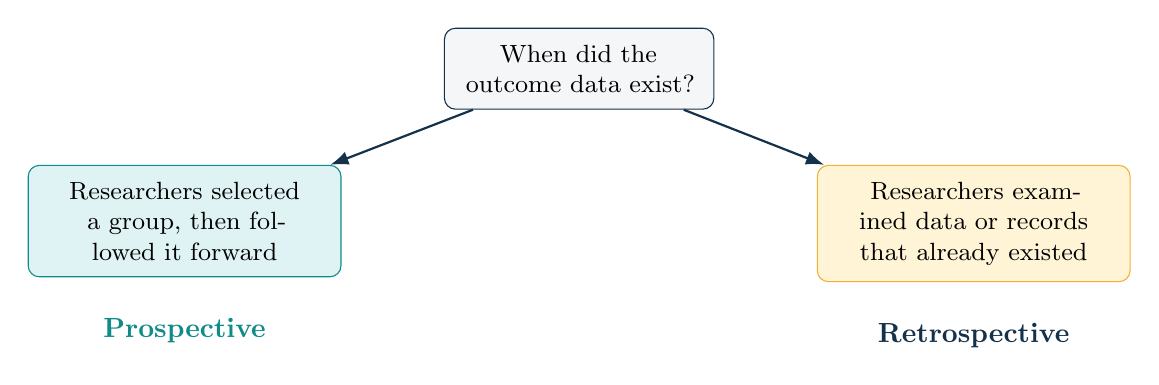
\begin{tikzpicture}[node distance=7mm and 13mm,every node/.style={font=\small}]
  \node[draw=Navy,rounded corners,fill=SoftGray,inner sep=6pt,text width=3.0cm,align=center] (q) {When did the outcome data exist?};
  \node[draw=Teal,rounded corners,fill=Sky,inner sep=6pt,text width=3.55cm,align=center,below left=of q] (p) {Researchers selected a group, then followed it forward};
  \node[draw=Gold,rounded corners,fill=GoldLight,inner sep=6pt,text width=3.55cm,align=center,below right=of q] (r) {Researchers examined data or records that already existed};
  \node[below=4mm of p,font=\bfseries\color{Teal}] {Prospective};
  \node[below=4mm of r,font=\bfseries\color{Navy}] {Retrospective};
  \draw[-{Latex},thick,Navy] (q) -- (p);
  \draw[-{Latex},thick,Navy] (q) -- (r);
\end{tikzpicture}
\end{center}

Valid limitations include unrepresentative sampling, inaccurate self-reports, a short observation period, and confounding. Observational evidence supports \emph{association}, not cause and effect.

\begin{answerbox}[Safe conclusion language]
Students who used one method \ans{tended to have higher scores}, or method and score \ans{were associated}. Do not say the method \emph{caused} higher scores unless a well-designed experiment justifies it.
\end{answerbox}

\subsection{Lesson 1.2: One and two categorical variables}

\begin{tabularx}{\textwidth}{>{\bfseries\color{Navy}}p{1.30in} Y Y}
\toprule
Display & Use & Rule\\
\midrule
Bar graph & Frequencies or relative frequencies for categories & Bars are separated; a frequency axis begins at 0.\\
Pie chart & Each category's share of one whole & Categories must be mutually exclusive and exhaustive, so the slices add to exactly $100\%$.\\
\bottomrule
\end{tabularx}

\begin{formulabox}{Frequency language}
\[
\text{relative frequency}=\frac{\text{category count}}{\text{total count}},\qquad
\text{percent}=100\%(\text{relative frequency}).
\]
Run it backward with
\[
\text{count}=(\text{proportion})(\text{total}),\qquad
\text{total}=\frac{\text{count}}{\text{proportion}}.
\]
From the notes, if 9 students are 30\% of a sample, then $n=9/0.30=\ans{30}$.
\end{formulabox}

\begin{trapbox}[Pie-chart check]
You may make a pie chart only when every individual belongs to exactly one category and the category percentages cover the entire group. The percentages must add to $100\%$. If categories overlap or the total is not $100\%$, do not use a pie chart.
\end{trapbox}

\subsubsection*{Two-way tables: choose the denominator first}

\begin{center}
\begin{tabular}{l|cc|c}
 & $B_1$ & $B_2$ & Total\\ \hline
$A_1$ & \cellcolor{CoralLight}$a$ & $b$ & \cellcolor{GoldLight}$a+b$\\
$A_2$ & $c$ & $d$ & \cellcolor{GoldLight}$c+d$\\ \hline
Total & \cellcolor{GoldLight}$a+c$ & \cellcolor{GoldLight}$b+d$ & \cellcolor{Sky}$n$\\
\end{tabular}
\end{center}

\begin{tabularx}{\textwidth}{>{\bfseries\color{Navy}}p{1.28in} Y p{2.10in}}
\toprule
Type & Clue & Denominator\\
\midrule
Marginal & One variable only & Grand total $n$\\
Joint & Two conditions joined by ``and'' & Grand total $n$\\
Conditional & ``of those who,'' ``among,'' or ``given'' & Total of the named given group\\
\bottomrule
\end{tabularx}

\begin{formulabox}{Same cell, different question}
\[
P(A_1)=\frac{a+b}{n},\qquad
P(A_1\text{ and }B_1)=\frac{a}{n},\qquad
P(A_1\mid B_1)=\frac{a}{a+c}.
\]
Underline the group after ``given'' or ``of those who'' before dividing.
\end{formulabox}

\begin{center}
\begin{tabular}{l|cc|c}
Favorite elective & Math & English & Total\\ \hline
Art & 2 & 4 & 6\\
Music & 5 & 4 & 9\\
P.E. & 4 & 3 & 7\\
World Language & 1 & 3 & 4\\
Technology & 4 & 0 & 4\\ \hline
Total & 16 & 14 & 30
\end{tabular}
\end{center}

\begin{tabularx}{\textwidth}{Y Y}
Percent of all students who chose P.E.:
\[\ans{7/30=23.3\%}\]
&
Percent who chose Math and Art:
\[\ans{2/30=6.7\%}\]\\
Percent who chose Technology, given Math:
\[\ans{4/16=25\%}\]
&
Percent who chose Math, given Technology:
\[\ans{4/4=100\%}\]
\end{tabularx}

\begin{trapbox}[Reverse condition]
$P(\text{Technology}\mid\text{Math})$ and $P(\text{Math}\mid\text{Technology})$ generally use different denominators. Also, a numerator may span several cells: ``private colleges'' may require adding private nonprofit and private for-profit.
\end{trapbox}

\subsection{Lesson 1.3: Association and categorical displays}

The \term{explanatory variable} may help explain or predict the \term{response variable}. To test for an association, compare the response distribution \emph{within each explanatory group}.

\begin{bigidea}{How to decide whether two categorical variables are associated}
\begin{enumerate}[label=\arabic*.]
  \item Choose the explanatory groups.
  \item Calculate the response percentages within each group.
  \item Compare corresponding conditional percentages.
  \item If the distributions differ meaningfully, state the association and give a specific contextual comparison.
\end{enumerate}
\end{bigidea}

\begin{answerbox}[Strong association sentence]
There \ans{is an association} between core-class preference and elective preference because the conditional distribution of elective preference differs by core-class group. For example, \ans{25\% of Math-preferring students chose Technology, compared with 0\% of English-preferring students}.
\end{answerbox}

\begin{tabularx}{\textwidth}{>{\bfseries\color{Navy}}p{1.43in} Y Y}
\toprule
Display & What it preserves & What to compare\\
\midrule
Side-by-side bars & Separate response bars within each group & Corresponding relative-frequency heights\\
Segmented bars & Equal-width, 100\%-tall group bars & Segment heights; counts across groups stay hidden\\
Mosaic plot & Heights are conditional proportions; widths show group sizes & Heights for association, widths for group size, areas for overall counts\\
\bottomrule
\end{tabularx}

\begin{formulabox}{Mosaic plot meanings}
\begin{align*}
\text{height}&=\text{conditional proportion},\\
\text{width}&=\text{group's share of the sample},\\
\text{area}&=\text{joint share of all individuals}.
\end{align*}
If a group contains five times as many individuals, its mosaic bar is five times as wide.
\end{formulabox}

Teachers and students voted for a mascot. There were 100 teachers and 500 students.

\begin{center}
\begin{tabular}{l|ccc|c}
 & Rams & Falcons & Prairie Dogs & Group size\\ \hline
Teachers & 80\% & 10\% & 10\% & 100\\
Students & 30\% & 60\% & 10\% & 500\\ \hline
Counts & \ans{$80+150=230$} & \ans{$10+300=310$} & \ans{$10+50=60$} & 600
\end{tabular}
\end{center}

Although Rams have the larger teacher percentage, Falcons win overall because the student group is much larger. Use $\text{count}=(\text{conditional proportion})(\text{group size})$.

\begin{trapbox}[Percent is not count]
A larger percentage need not mean a larger count when group sizes differ. Segmented bars hide group sizes; a mosaic plot reveals them through widths. Without group sizes, do not compare counts across different segmented bars.
\end{trapbox}

Misleading displays may truncate a bar graph's vertical axis, scale pictures in both height and width, use unequal intervals, or invite invalid count comparisons. A corrected frequency bar graph begins at 0.

\section{Lesson 1.4: Describing Quantitative Data}

\begin{bigidea}{Choose a display that matches the question}
Dotplots and stem-and-leaf plots preserve individual values. Histograms group values into intervals and make the overall shape easier to see. A stem-and-leaf plot must include a key, such as $5\mid2=52$.
\end{bigidea}

\begin{tabularx}{\textwidth}{>{\bfseries\color{Navy}}p{1.35in} Y Y}
\toprule
Display & Best feature & Limitation\\
\midrule
Dotplot & Exact values, clusters, gaps, and possible outliers & Crowded for large data sets\\
Stem-and-leaf & Exact ordered values and overall shape & Awkward with many values or wide scales\\
Histogram & Shape of a large quantitative distribution & Exact observations are hidden; bars touch\\
\bottomrule
\end{tabularx}

\begin{trapbox}[Bar graph or histogram?]
A bar graph is for categorical data and its bars are separated. A histogram is for quantitative data grouped into intervals and its bars touch. The horizontal order in a histogram is numerical and cannot be rearranged.
\end{trapbox}

\subsection{SOCV: the complete description}

Always describe a quantitative distribution with \term{Shape, Outliers, Center, Variability}, in context.

\begin{tabularx}{\textwidth}{>{\bfseries\color{Navy}}p{0.95in} Y p{2.25in}}
\toprule
Letter & What to report & Vocabulary / measure\\
\midrule
S & Overall shape & symmetric; skewed left/right; unimodal, bimodal, or uniform; clusters and gaps\\
O & Unusual values & possible outliers, with approximate values\\
C & Typical value & mean when symmetric/no strong outliers; median when skewed/outliers\\
V & Amount of spread & range, IQR, or SD, with units\\
\bottomrule
\end{tabularx}

\begin{center}
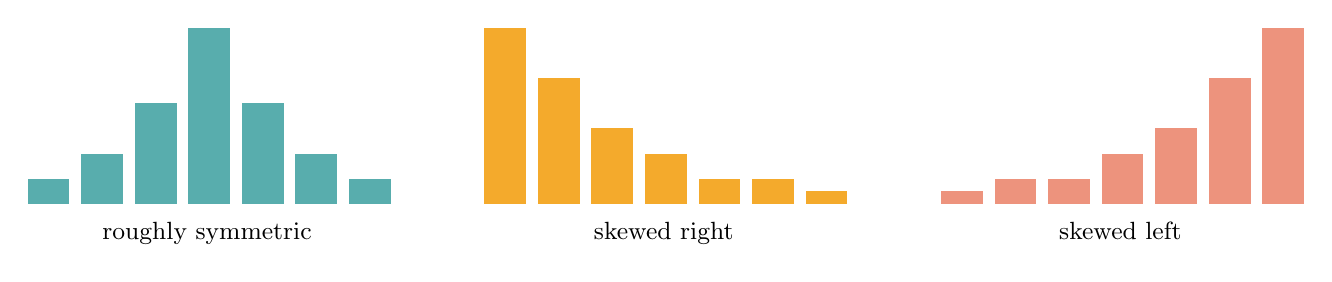
\begin{tikzpicture}[x=0.68cm,y=0.32cm,font=\small]
  \foreach \x/\h in {0/1,1/2,2/4,3/7,4/4,5/2,6/1}{\fill[Teal!70] (\x,0) rectangle +(0.78,\h);}
  \node[below] at (3.35,-0.35) {roughly symmetric};
  \begin{scope}[xshift=5.8cm]
    \foreach \x/\h in {0/7,1/5,2/3,3/2,4/1,5/1,6/0.5}{\fill[Gold!85!orange] (\x,0) rectangle +(0.78,\h);}
    \node[below] at (3.35,-0.35) {skewed right};
  \end{scope}
  \begin{scope}[xshift=11.6cm]
    \foreach \x/\h in {0/0.5,1/1,2/1,3/2,4/3,5/5,6/7}{\fill[Coral!75] (\x,0) rectangle +(0.78,\h);}
    \node[below] at (3.35,-0.35) {skewed left};
  \end{scope}
\end{tikzpicture}
\end{center}

\key{Tail direction names the skew.} A few large values create a right tail; a few small values create a left tail.

\begin{answerbox}[Model SOCV description]
The backpack-weight distribution is \ans{roughly symmetric and unimodal}, with \ans{no obvious outliers}. Its center is about \ans{6.5 pounds} and its values range from \ans{4 to 10 pounds}, a range of \ans{6 pounds}.
\end{answerbox}

\begin{trapbox}[Do not give a number without context]
Write ``The median backpack weight is 6.5 pounds,'' not merely ``the center is 6.5.'' For a graph, use approximate language when exact values are not available.
\end{trapbox}

\section{Lesson 1.5: Measuring Center and Variability}

\begin{formulabox}{Core measures}
\begin{align*}
\bar{x}&=\frac{\sum x_i}{n},
&\text{range}&=\max-\min,\\
s&=\sqrt{\frac{\sum (x_i-\bar{x})^2}{n-1}},
&\text{variance}&=s^2.
\end{align*}
The sample standard deviation $s$ measures the typical distance of the observations from the sample mean $\bar{x}$.
\end{formulabox}

\begin{answerbox}[Correct SD interpretation]
For the five reported weekly work times, $s=9.86$ hours means the parents' reported work times \ans{typically vary by about 9.86 hours from the mean of 43.6 hours}.
\end{answerbox}

\begin{trapbox}[What SD is not]
SD is not the average value, not the range, and not a statement that every observation lies exactly $s$ units from the mean. It is never negative and is 0 only when all values are equal.
\end{trapbox}

\subsection{Choose matching measures}

\begin{tabularx}{\textwidth}{>{\bfseries\color{Navy}}p{1.65in} Y Y}
\toprule
Distribution & Center & Spread\\
\midrule
Roughly symmetric with no strong outliers & Mean $\bar{x}$ & Standard deviation $s$\\
Skewed or containing outliers & Median & IQR\\
\bottomrule
\end{tabularx}

\begin{bigidea}{Resistance}
The \term{median} and \term{IQR} are resistant: a few extreme values have limited effect. The \term{mean}, \term{SD}, and \term{range} are nonresistant: an extreme value can change them substantially.
\end{bigidea}

\begin{tabularx}{\textwidth}{>{\bfseries\color{Navy}}p{1.52in} C C C}
\toprule
Shape & Skewed left & Symmetric & Skewed right\\
\midrule
Mean vs. median & mean $<$ median & mean $\approx$ median & mean $>$ median\\
Reason & low tail pulls mean left & balanced tails & high tail pulls mean right\\
\bottomrule
\end{tabularx}

For the provided rainfall data, mean $=34.94$, median $=40.5$, and $s=15.52$. Since mean $<$ median, the distribution is skewed left; the small observations pull the mean toward the left tail.

\subsection{Reasoning about SD without calculation}

SD is larger when observations lie farther from the mean. The sets
\[
A=\{40,45,50,55,60\},\qquad B=\{46,48,50,52,54\}
\]
have the same mean and median, but $A$ has the larger SD because its values are more spread out.

If a value equal to the current mean is added, the mean stays the same and the SD usually decreases: the sum of squared deviations stays the same while the denominator increases.

\section{Lesson 1.6: Comparing Quantitative Data}

\subsection{Quartiles and the five-number summary}

The five-number summary is
\[
\min,\quad Q_1,\quad \text{median},\quad Q_3,\quad \max.
\]
$Q_1$ is the median of the lower half and $Q_3$ is the median of the upper half, using the class convention. Each quartile section contains about 25\% of the observations, and about 50\% lie between $Q_1$ and $Q_3$.

\begin{formulabox}{IQR and the $1.5\times IQR$ outlier rule}
\[
IQR=Q_3-Q_1
\]
\[
\text{lower fence}=Q_1-1.5(IQR),\qquad
\text{upper fence}=Q_3+1.5(IQR).
\]
Any observation below the lower fence or above the upper fence is an outlier by this rule. A second rule from the notes flags values below $\bar{x}-2s$ or above $\bar{x}+2s$.
\end{formulabox}

For the lacrosse goals data, $Q_1=6$, median $=13$, $Q_3=32$, mean $=27$, and $s=35.12$.
\[
IQR=26,\quad 6-1.5(26)=-33,\quad 32+1.5(26)=71.
\]
Thus 107 and 121 are high outliers. The $2s$ interval is
\[
27\pm2(35.12)=[-43.24,97.24],
\]
which flags the same two values.

\subsection{Modified boxplots}

A modified boxplot draws the box from $Q_1$ to $Q_3$, a line at the median, whiskers to the most extreme \emph{non-outliers}, and separate points for outliers.

\begin{center}
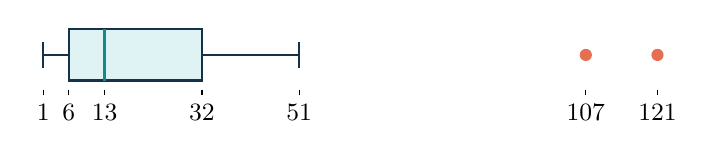
\begin{tikzpicture}[x=0.065cm,y=0.65cm,font=\small]
  \draw[thick,Navy] (1,0)--(6,0);
  \draw[thick,Navy] (32,0)--(51,0);
  \draw[thick,Navy,fill=Sky] (6,-0.5) rectangle (32,0.5);
  \draw[very thick,Teal] (13,-0.5)--(13,0.5);
  \draw[thick,Navy] (1,-0.25)--(1,0.25);
  \draw[thick,Navy] (51,-0.25)--(51,0.25);
  \fill[Coral] (107,0) circle (2.2pt);
  \fill[Coral] (121,0) circle (2.2pt);
  \foreach \x in {1,6,13,32,51,107,121}{\draw (\x,-0.68)--(\x,-0.78) node[below] {\x};}
\end{tikzpicture}
\end{center}

\begin{trapbox}[Whiskers do not always reach min and max]
In a modified boxplot, the whiskers stop at the smallest and largest non-outliers. Plot each outlier separately. Boxplots show quartiles and outliers well, but they hide individual values, clusters, and gaps that a dotplot can reveal.
\end{trapbox}

\subsection{Compare distributions with SOCV}

Use comparative words such as \emph{higher}, \emph{lower}, \emph{more variable}, and \emph{less variable}. Do not describe each group in isolation.

\begin{answerbox}[Model comparison]
Both calorie distributions are \ans{roughly symmetric} with \ans{no apparent outliers}. Sandwiches have a \ans{higher median, about 830 calories, versus about 475 for salads}. Sandwich calories are also \ans{more variable}, with an IQR of about \ans{340 calories} compared with about \ans{180 calories} for salads.
\end{answerbox}

\begin{trapbox}[Histogram precision]
A histogram usually does not reveal the exact median or quartiles because values are grouped into intervals. It may support an interval estimate, such as ``$Q_1$ lies between 40\% and 50\%.''
\end{trapbox}

\section{Lesson 1.7: Location in a Distribution}

\subsection{Percentiles}

The $p$th percentile is a value with about $p\%$ of observations at or below it.

\begin{formulabox}{Percentile of an observed value}
\[
\text{percentile}=\frac{\#\text{ observations at or below the value}}{n}(100\%).
\]
Use the counting convention from class. A percentile is a relative position, not the percent correct on a test.
\end{formulabox}

If 7 of 16 recorded sleep times are at or below 119 minutes, then 119 minutes is at the
\[
\ans{\frac{7}{16}(100\%)=43.75\%\approx44\text{th percentile}.}
\]

\begin{answerbox}[Correct percentile interpretation]
A child at the 65th percentile for weight weighs \ans{at least as much as about 65\% of children of the same age and sex}. It does not mean the child weighs 65\% more or that the weight is 65\% of a maximum.
\end{answerbox}

\subsection{Standard scores (z-scores)}

\begin{formulabox}{Standardized location}
\[
z=\frac{x-\bar{x}}{s},\qquad x=\bar{x}+zs.
\]
$z>0$ means above the mean, $z<0$ means below the mean, and $|z|$ is the distance from the mean in standard deviations.
\end{formulabox}

For a quiz with mean 80 and SD 10, a score of 65 has
\[
z=\frac{65-80}{10}=\ans{-1.5}.
\]
Interpretation: the score of 65 is \ans{1.5 standard deviations below the mean}.

\begin{bigidea}{Comparing different distributions}
Compare relative standing with $z$-scores, not raw values. The higher $z$-score has the higher relative position. The value farther from its mean has the larger $|z|$.
\end{bigidea}

From the salary homework, a business salary of $\$72{,}000$ has
\[
z=\frac{72-69.929}{5.954}\approx\ans{0.35},
\]
while a communications salary of $\$65{,}000$ has
\[
z=\frac{65-56.467}{6.632}\approx\ans{1.29}.
\]
The $\$65{,}000$ communications salary is lower in raw dollars but higher relative to its major.

\begin{trapbox}[Sign vs. distance]
To find which value is \emph{higher relative to its group}, compare signed $z$-scores. To find which is \emph{farther from the mean}, compare absolute values $|z|$.
\end{trapbox}

\section{Lesson 1.8: Linear Transformations}

Suppose every observation is transformed by
\[
y=a+bx.
\]

\begin{bigidea}{Transformation rule}
Adding or subtracting changes location but not spread. Multiplying or dividing changes both location and spread. For the positive multipliers used in these lessons, the distribution's shape stays the same.
\end{bigidea}

\begin{tabularx}{\textwidth}{>{\bfseries\color{Navy}}p{1.55in} Y Y}
\toprule
Feature & Add $a$ & Multiply by $b>0$\\
\midrule
Shape & unchanged & unchanged\\
Mean, median, quartiles & add $a$ & multiply by $b$\\
Range, IQR, SD & unchanged & multiply by $b$\\
Variance & unchanged & multiply by $b^2$\\
$z$-scores & unchanged & unchanged\\
Outlier status & unchanged & unchanged\\
\bottomrule
\end{tabularx}

In full generality, spreads are multiplied by $|b|$; if $b<0$, the order reverses and the shape is reflected.

\begin{formulabox}{Summary statistics under $y=a+bx$}
\[
\bar{y}=a+b\bar{x},\qquad
\operatorname{median}(y)=a+b\operatorname{median}(x),\qquad
s_y=|b|s_x,
\]
\[
IQR_y=|b|IQR_x,\qquad
\operatorname{Var}(y)=b^2\operatorname{Var}(x).
\]
Apply the addition to center measures only; do not add it to SD, range, or IQR.
\end{formulabox}

\subsection{Worked taxi transformation}

Taxi cost is $C=5+3.25d$, where $d$ is distance in miles. The distance summary has $\bar{d}=6.75$, $s_d=6.61$, $Q_1=2.5$, median $=3.5$, and $Q_3=10.5$.

\begin{align*}
\bar{C}&=5+3.25(6.75)=\ans{\$26.94},\\
s_C&=3.25(6.61)=\ans{\$21.48},\\
Q_{1,C}&=5+3.25(2.5)=\ans{\$13.125},\\
Q_{3,C}&=5+3.25(10.5)=\ans{\$39.125}.
\end{align*}

The original $IQR=8$, so the upper distance fence is $10.5+1.5(8)=22.5$ miles. A 23-mile ride is an outlier. Its cost is $5+3.25(23)=\$79.75$, and the transformed upper fence is $5+3.25(22.5)=\$78.125$, so it remains an outlier.

\subsection{Standardizing a distribution}

Standardizing transforms every value into its $z$-score:
\[
z=\frac{x-\bar{x}}{s}=-\frac{\bar{x}}{s}+\frac{1}{s}x.
\]
The standardized distribution has the \key{same shape}, \key{mean 0}, and \key{SD 1}. A positive unit conversion also leaves every $z$-score unchanged.

\begin{trapbox}[Variance squares the multiplier]
If SD is multiplied by 12, variance is multiplied by $12^2=144$. For egg sales with SD 3 dozen, variance is $9$ dozen$^2$. Converting to individual eggs gives SD $36$ eggs and variance $1296$ eggs$^2$.
\end{trapbox}

\newpage
\section{Master Decision and Formula Sheet}

\begin{tabularx}{\textwidth}{>{\bfseries\color{Navy}}p{2.05in} Y}
\toprule
When the question asks... & Do this\\
\midrule
Category share of a whole & Relative frequency; use a pie chart only if mutually exclusive, exhaustive shares total 100\%.\\
``of all'' with one category & Marginal proportion; divide by grand total.\\
``of all'' with ``and'' & Joint proportion; divide by grand total.\\
``among,'' ``given,'' ``of those who'' & Conditional proportion; denominator is the named group.\\
Whether categorical variables are associated & Compare complete conditional distributions; cite one specific difference.\\
Whether counts differ across percentage bars & Need group sizes; multiply proportion by group size.\\
Describe one quantitative distribution & SOCV, in context.\\
Choose center and spread & Symmetric/no outlier: mean and SD. Skewed/outlier: median and IQR.\\
Find outliers & Calculate IQR, fences, then compare every extreme value to the fences.\\
Draw a modified boxplot & Box at $Q_1,Q_3$, median line, whiskers to non-outliers, outliers as points.\\
Compare quantitative groups & Compare shape, unusual features, center, and variability using comparative words and units.\\
Find relative position & Percentile for percent at/below; $z$-score for SDs above/below mean.\\
Transform every value & Apply $a+b x$ to center; multiply spread by $|b|$; multiply variance by $b^2$.\\
\bottomrule
\end{tabularx}

\begin{multicols}{2}
\begin{formulabox}{Categorical data}
\small
\[
\text{relative frequency}=\frac{\text{count}}{\text{total}}
\]
\[
\text{count}=(\text{proportion})(\text{group size})
\]
\[
P(A\mid B)=\frac{\#(A\text{ and }B)}{\#B}
\]
\end{formulabox}

\begin{formulabox}{Quantitative data}
\small
\[
\bar{x}=\frac{\sum x_i}{n},\quad
s=\sqrt{\frac{\sum(x_i-\bar{x})^2}{n-1}}
\]
\[
IQR=Q_3-Q_1
\]
\[
Q_1-1.5IQR,\quad Q_3+1.5IQR
\]
\[
z=\frac{x-\bar{x}}{s},\quad x=\bar{x}+zs
\]
\end{formulabox}
\end{multicols}

\section{Seven Essential Practice Questions}

These are the highest-yield question types across the provided materials. Complete them without looking at the answer key.

\subsection*{1. Study design and variables}
Researchers randomly select 400 juniors from a school district. At the beginning of the semester, students report their main study method (flashcards, practice tests, or videos). At the end of the semester, researchers record each student's final exam score.

\begin{enumerate}[label=\alph*.]
  \item Identify the population and sample.
  \item Identify both variables and classify each as categorical or quantitative.
  \item Is the study prospective or retrospective? Explain.
  \item State one limitation and write a conclusion that does not claim causation.
\end{enumerate}
\longwork

\subsection*{2. Two-way table, association, and displays}
The results for another sample are shown below.

\begin{center}
\begin{tabular}{l|cc|c}
Study method & Passed & Did not pass & Total\\ \hline
Flashcards & 36 & 12 & 48\\
Practice tests & 54 & 6 & 60\\
Videos & 20 & 12 & 32\\ \hline
Total & 110 & 30 & 140
\end{tabular}
\end{center}

\begin{enumerate}[label=\alph*.]
  \item Find the marginal percent who used practice tests.
  \item Find the joint percent who used videos and did not pass.
  \item Find the percent who passed, given flashcards.
  \item Find the percent who used flashcards, given that they passed.
  \item Is there an association between study method and passing? Support your answer with conditional percentages.
  \item Could study method be displayed in a pie chart? State the exact condition that makes your answer valid.
  \item In a mosaic plot, give the width ratio for the three study-method bars.
\end{enumerate}
\longwork

\newpage
\subsection*{3. Display and SOCV}
The number of late assignments for 10 students is
\[
4,\ 4,\ 5,\ 6,\ 6,\ 6,\ 7,\ 8,\ 9,\ 14.
\]

\begin{enumerate}[label=\alph*.]
  \item Is this variable categorical, quantitative discrete, or quantitative continuous?
  \item Find the mean, median, and range.
  \item Find $Q_1$, $Q_3$, and IQR, then use the $1.5\times IQR$ rule to check 14.
  \item Describe the distribution with SOCV. Which center and spread would you report?
  \item Which display, a dotplot or histogram, better preserves every individual value?
\end{enumerate}
\longwork

\subsection*{4. Standard deviation and resistance}
Five parents report weekly work times of
\[
38,\ 45,\ 60,\ 40,\ 35\text{ hours}.
\]
The mean is 43.6 hours and the sample SD is 9.86 hours.

\begin{enumerate}[label=\alph*.]
  \item Interpret the standard deviation in context.
  \item If 60 is replaced by 120, predict what happens to the mean, median, range, and SD. Explain briefly.
  \item After that replacement, which pair should summarize the data: mean and SD, or median and IQR?
\end{enumerate}
\longwork

\subsection*{5. Outliers and a modified boxplot}
For lacrosse goals, $Q_1=6$, median $=13$, $Q_3=32$, mean $=27$, and $s=35.12$. The largest observations are 50, 51, 107, and 121; the minimum is 1.

\begin{enumerate}[label=\alph*.]
  \item Use the $1.5\times IQR$ rule to identify high outliers.
  \item Use the $2s$ rule to identify high outliers.
  \item State the endpoints of the whiskers and list the separately plotted points in a modified boxplot.
  \item Predict the shape and explain why the mean is much larger than the median.
\end{enumerate}
\longwork

\newpage
\subsection*{6. Percentiles and z-scores}
\begin{enumerate}[label=\alph*.]
  \item In a list of 20 ordered scores, 15 are at or below Maya's score. Find and interpret Maya's percentile.
  \item Quiz A has mean 80 and SD 10. Find and interpret the $z$-score for 65.
  \item Quiz B has mean 72 and SD 6. Find the $z$-score for 81. Which student has the higher relative standing: the 65 on Quiz A or the 81 on Quiz B?
  \item On Quiz A, what raw score has $z=-0.3$?
  \item Two values have $z$-scores $1.4$ and $-2.1$. Which is at the higher percentile? Which is farther from its mean?
\end{enumerate}
\longwork

\subsection*{7. Linear transformation}
Taxi cost is $C=5+3.25d$, where distance $d$ is in miles. For a set of rides,
\[
\bar d=6.75,\quad s_d=6.61,\quad Q_1=2.5,\quad \text{median}=3.5,\quad Q_3=10.5,
\]
and the longest ride is 23 miles.

\begin{enumerate}[label=\alph*.]
  \item Find the mean and SD of the costs.
  \item Find $Q_1$, the median, $Q_3$, and IQR of the costs.
  \item Use the distance summary to decide whether 23 miles is an outlier. Then verify that its cost, $\$79.75$, is also an outlier on the cost scale.
  \item What happens to the shape and all $z$-scores?
  \item If another variable with variance 9 is multiplied by 12, what is its new variance?
\end{enumerate}
\longwork

\newpage
\section{Answer Key and Explanations}

\subsection*{1. Study design and variables}
\begin{answerbox}
\begin{enumerate}[label=\alph*.]
  \item \ans{Population: all juniors in the school district. Sample: the 400 randomly selected juniors.}
  \item \ans{Main study method is categorical; final exam score is quantitative.}
  \item \ans{Prospective, because students were selected and reported their method before researchers recorded a future exam outcome.}
  \item \ans{One limitation is that study method is self-reported or that other variables, such as previous achievement, may confound the relationship. Safe conclusion: in this sample, study method was associated with final exam score; students using one method tended to score differently. The observational study does not prove the method caused the difference.}
\end{enumerate}
\end{answerbox}

\subsection*{2. Two-way table, association, and displays}
\begin{answerbox}
\begin{enumerate}[label=\alph*.]
  \item \ans{$60/140=0.4286=42.9\%$.}
  \item \ans{$12/140=0.0857=8.6\%$.}
  \item \ans{$36/48=0.75=75\%$.}
  \item \ans{$36/110=0.3273=32.7\%$.} Same cell, different denominator from part (c).
  \item \ans{Yes. Pass rates are flashcards $36/48=75\%$, practice tests $54/60=90\%$, and videos $20/32=62.5\%$. The conditional distribution of passing differs by method. This is association, not proof of causation.}
  \item \ans{Yes, if each student selected exactly one of the three methods and the three categories cover the full sample. Then their shares are mutually exclusive and exhaustive and add to $100\%$.}
  \item \ans{$48:60:32$, which simplifies to $12:15:8$. Mosaic widths are proportional to group sizes.}
\end{enumerate}
\end{answerbox}

\subsection*{3. Display and SOCV}
\begin{answerbox}
\begin{enumerate}[label=\alph*.]
  \item \ans{Quantitative discrete, because this is a count.}
  \item \ans{$\bar{x}=69/10=6.9$ assignments; median $=(6+6)/2=6$; range $=14-4=10$.}
  \item \ans{$Q_1=5$, $Q_3=8$, so $IQR=3$. The fences are $5-1.5(3)=0.5$ and $8+1.5(3)=12.5$. Since $14>12.5$, 14 is a high outlier.}
  \item \ans{The distribution is unimodal and skewed right, with a high outlier at 14. Its center is about 6 late assignments. Because of the skew and outlier, report median $=6$ and IQR $=3$ assignments.}
  \item \ans{A dotplot preserves every individual value.}
\end{enumerate}
\end{answerbox}

\subsection*{4. Standard deviation and resistance}
\begin{answerbox}
\begin{enumerate}[label=\alph*.]
  \item \ans{The reported weekly work times typically vary by about 9.86 hours from their mean of 43.6 hours.}
  \item \ans{The mean increases because the total increases; the sorted data become $35,38,40,45,120$, so the median remains 40. The range increases from $60-35=25$ to $120-35=85$, and SD increases because 120 lies much farther from the mean.}
  \item \ans{Median and IQR, because the extreme value makes the distribution right-skewed and those measures are resistant.}
\end{enumerate}
\end{answerbox}

\subsection*{5. Outliers and a modified boxplot}
\begin{answerbox}
\begin{enumerate}[label=\alph*.]
  \item \ans{$IQR=32-6=26$. The upper fence is $32+1.5(26)=71$, so 107 and 121 are high outliers. The lower fence is $-33$.}
  \item \ans{$\bar{x}+2s=27+2(35.12)=97.24$, so 107 and 121 are high outliers. The lower cutoff is $-43.24$.}
  \item \ans{Left whisker at 1 and right whisker at 51; plot 107 and 121 separately.}
  \item \ans{Strongly skewed right. The two very large goal totals pull the nonresistant mean upward, while the resistant median changes much less.}
\end{enumerate}
\end{answerbox}

\subsection*{6. Percentiles and z-scores}
\begin{answerbox}
\begin{enumerate}[label=\alph*.]
  \item \ans{$15/20=75\%$, so Maya is at the 75th percentile: about 75\% of the scores are at or below hers.}
  \item \ans{$z=(65-80)/10=-1.5$. The score is 1.5 SD below the Quiz A mean.}
  \item \ans{$z=(81-72)/6=1.5$. The Quiz B student has the higher relative standing because $1.5>-1.5$.}
  \item \ans{$x=80+(-0.3)(10)=77$.}
  \item \ans{The value with $z=1.4$ is at the higher percentile. The value with $z=-2.1$ is farther from its mean because $|-2.1|>|1.4|$.}
\end{enumerate}
\end{answerbox}

\Needspace{0.40\textheight}
\subsection*{7. Linear transformation}
\begin{answerbox}
\begin{enumerate}[label=\alph*.]
  \item \ans{$\bar C=5+3.25(6.75)=\$26.9375\approx\$26.94$; $s_C=3.25(6.61)=\$21.4825\approx\$21.48$. Do not add $\$5$ to SD.}
  \item \ans{$Q_1=5+3.25(2.5)=\$13.125$; median $=5+3.25(3.5)=\$16.375$; $Q_3=5+3.25(10.5)=\$39.125$; $IQR=3.25(8)=\$26$.}
  \item \ans{Distance upper fence: $10.5+1.5(8)=22.5$ miles, so 23 miles is an outlier. Cost upper fence: $39.125+1.5(26)=\$78.125$, and $\$79.75>\$78.125$, so the transformed value is also an outlier.}
  \item \ans{The positive linear transformation preserves the shape and every $z$-score.}
  \item \ans{$12^2(9)=144(9)=1296$. Variance uses the square of the multiplier.}
\end{enumerate}
\end{answerbox}

\begin{tcolorbox}[colback=Navy,colframe=Navy,arc=2mm,boxrule=0pt]
\centering
{\large\bfseries\color{white} Final self-check}\par
\color{white}Can you choose the denominator, describe with SOCV, pair center with spread, interpret a $z$-score, and transform center and spread differently? If yes, you are ready.
\end{tcolorbox}

\end{document}
